\section{Evaluation}
For the quality control of the workflow, we first evaluate the segmentation process and then the registration.
The segmentations of the classifier should be as precise as possible for the masking process, which in return is then used to improve the registration.

As stated by Ioanas et al. in TODO:cite a major challenge of registration QC is that a perfect mapping from the measured image to the template is undefined.
To address this challenge, they developed four alternative evaluation metrics: volume conservation, smoothness conservation, functional analysis, and variance analysis.
We will use these metrics to benchmark our workflow against theirs.

\subsection{Segmentation}
Quality control of our classifier is difficult in the sense that it should predict a better mask than the template.
Nevertheless, it is use-full to verify if the output is similar, as it should be.
As a similarity metric we have used the Dice score (see \cref{eqDcoef}).
The median Dice score taken on every slice of the test data set is $D_{coef}= $ \py{boilerplate.print_dice()} $\sim 1$.
The prediction thus have only minor changes in comparison with the template, which should represent small improvements.

\begin{sansmath}
\py{pytex_subfigs(
        [
                {'script':'scripts/classifier/plot_test_corr_df.py', 'label':'subfig:test_corr','conf':'article/1col.conf', 'options_pre':'{.48\\textwidth} \\vspace{-2em}',
                        'options_pre_caption':'\\vspace{-1.5em}',
                        'options_post':'\\vspace{1em}',
                        'label':'subfig:test_corr',
                        'caption':'Cross Correlations between the Test Set and the predictions.'
                        ,},
                {'script':'scripts/classifier/plot_bl_corr.py', 'label':'subfig:bl_corr','conf':'article/1col.conf', 'options_pre':'{.48\\textwidth}',
                        'options_pre_caption':'\\vspace{-1.5em}\\',
                        'options_post':'\\vspace{1em}',
                        'caption':'Cross Correlations between the blacklisted slices and the predictions.'
                        ,},
                ],
        caption='\\textbf{Overall the predictions of the classifier correlate better with the images, when taking the blacklisted slices into account.}
        Two tables comparing the correlation of the classifiers prediction and the template mask with the images.
        ',
        label='fig:corr',
        )}
\end{sansmath}


It is hard to measure how much better the predicted masks from the classifier are, compared with the template, because both are very accurate.
They both correlate similarily with the images for example, as can be seen in \cref{subfig:test_corr}:
\py{boilerplate.print_testcorr_ytrue()} against \py{boilerplate.print_testcorr_ypred()}.

Where the classifier clearly has the advantage is on the blacklisted slices.
Due to the data agumentation on the training set, the classifier is trained to predict well on incongruent data and thus has a better correlation with the blacklisted slices than the template (\py{boilerplate.print_blcorr_ypred()} against \py{boilerplate.print_blcorr_ytrue()}).
Here the argument could be brought that one could do the inverse: taking all the bad predictions of the classifier and comparing them to the template.
However, in total, the classifier has less predicitons with a lower correlation than: compared to the template: TODO


%\begin{figure}
%    \centering
%    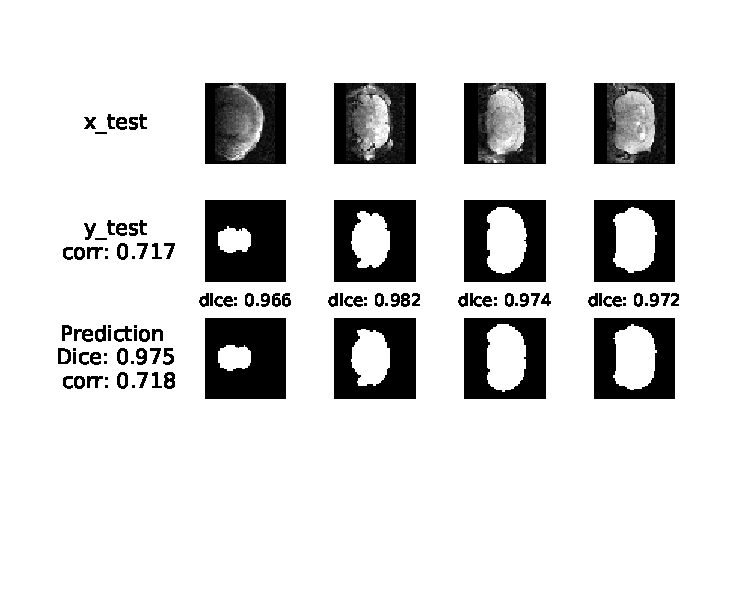
\includegraphics{mlebe_figs/sub-6542_ses-ofMaF_acq-TurboRARE_T2w1.pdf}
%    \caption{Caption}
%    \label{fig:my_label}
%\end{figure}


As an evaluation of the registration, we make use of the quality control from TODO:cite

\subsection{Volume Conservation}

\begin{sansmath}
\py{pytex_subfigs(
        [
                {'script':'scripts/vcc_violin.py', 'label':'vccv','conf':'article/1col.conf', 'options_pre':'{.48\\textwidth} \\vspace{-2em}',
                        'options_pre_caption':'\\vspace{-1.5em}',
                        'options_post':'\\vspace{1em}',
                        'caption':'Comparison across workflows and functional contrasts, considering only matching template-workflow combinations.'
                        ,},
                {'script':'scripts/scf_violin_contrasts.py', 'label':'sccv','conf':'article/1col.conf', 'options_pre':'{.48\\textwidth}',
                        'options_pre_caption':'\\vspace{-1.5em}\\',
                        'options_post':'\\vspace{1em}',
                        'caption':'Comparison across workflows and functional contrasts, considering only matching template-workflow combinations.'
                        ,},
                        {'script':'scripts/msc_violin.py', 'label':'mscv','conf':'article/1col.conf', 'options_pre':'{.48\\textwidth}',
                        'options_pre_caption':'\\vspace{-1.5em}',
                        'caption':'Comparison across workflows and functional contrasts, considering only matching template-workflow combinations.'
                        ,},
                ],
        caption='\\textbf{The SAMRI Generic workflow and template optimally and reliably conserve volume and smoothness --- unlike the Legacy workflow and template.}
        Plots of three target metrics, with coloured patch widths estimating distribution density, solid lines indicating the sample mean, and dashed lines indicate the inner quartiles.
        ',
        label='fig:vc',
        )}
\end{sansmath}

Volume conservation is based on the assumption that the total volume of the scanned segment of the brain should remain roughly constant after preprocessing.
Beyond just size differences between the acquired data and the target template, a volume increase may indicate that the brain was stretched to fill in template brain space not covered by the scan, while a volume decrease might indicate that non-brain voxels were introduced into the template brain space.
For this analysis we compute a Volume Conservation Factor (VCF), whereby volume conservation is highest for a VCF equal to 1.

%As seen in \cref{fig:vcv},
we note that in the described dataset VCF is sensitive to
the workflow (\py{boilerplate.fstatistic('Processing', condensed=True)}),
%the template (\py{boilerplate.fstatistic('Template', condensed=True)}),
%but not the interaction thereof (\py{boilerplate.fstatistic('Processing:Template', condensed=True)}).

The performance of the Generic SAMRI workflow in conjunction with the Generic template is significantly different from that of the Generic SAMRI workflow with the additional masking node, yielding a two-tailed p-value of \py{pytex_printonly('scripts/vc_t.py')}.
Moreover, the root mean squared error ratio strongly favours the Generic workflow
\\
\\
($\mathrm{RMSE_{GM}/RMSE_{G}\simeq} \py{pytex_printonly('scripts/vc_rmser.py')}$).
\\
\\


Descriptively, we observe that the Generic level of the template variable introduces a notable volume loss
(VCF of  ?? %\py{boilerplate.factorci('Template[T.Legacy]')}),
while the Legacy level of the workflow variable introduces a volume gain
(VCF of \py{boilerplate.factorci('Processing[T.Generic Masked]')}).
%Further, we note that there is a very strong variance increase in all conditions for the Legacy workflow
%(\py{boilerplate.varianceratio(template='Legacy')}-fold given the Legacy template, and \py{boilerplate.varianceratio(template='Generic')}-fold given the Generic template).



With respect to the data break-up by contrast (CBV versus BOLD, \cref{fig:vccv}), we see no notable main effect for the contrast variable
(VCF of \py{boilerplate.corecomparison_factorci('Contrast[T.CBV]')}).
%We do, however, report a notable effect for the contrast-template interaction, with the Legacy workflow and CBV contrast interaction level introducing a volume loss
%(VCF of \py{boilerplate.corecomparison_factorci('Processing[T.Legacy]:Contrast[T.CBV]')}).



\subsection{Smoothness Conservation}

A further aspect of preprocessing quality is the resulting image smoothness.
Although controlled smoothing is a valuable preprocessing tool used to increase the signal-to-noise ratio (SNR), uncontrolled smoothness limits operator discretion in the trade-off between SNR and feature granularity.
Uncontrolled smoothness can thus lead to undocumented and implicit loss of spatial resolution and is therefore associated with inferior anatomical alignment \cite{fmriprep}.
We employ a Smoothness Conservation Factor (SCF), expressing the ratio between the smoothness of the preprocessed images and the smoothness of the original images.

With respect to the data shown in \cref{fig:scv}, we note that SCF is sensitive to
%the template (\py{boilerplate.fstatistic('Template', condensed=True, df_path='data/smoothness.csv', dependent_variable='Smoothness Conservation Factor')}),
the workflow (\py{boilerplate.fstatistic('Processing', condensed=True, df_path='data/smoothness.csv', dependent_variable='Smoothness Conservation Factor')}),
%and the interaction of the factors (\py{boilerplate.fstatistic('Processing:Template', condensed=True, df_path='data/smoothness.csv', dependent_variable='Smoothness Conservation Factor')}).

The performance of the Generic SAMRI workflow in conjunction with the Generic template is significantly different from that of the Legacy workflow in conjunction with the Legacy template, yielding a two-tailed p-value of \py{pytex_printonly('scripts/scf_t.py')}.
In this comparison, the root mean squared error ratio favours the Generic workflow
\\
\\
($\mathrm{RMSE_{GM}/RMSE_{G}\simeq} \py{pytex_printonly('scripts/scf_rmser.py')}$).
\\
\\

Descriptively, we observe that the Legacy level of the template variable introduces a smoothness reduction
%(SCF of \py{boilerplate.factorci('Template[T.Legacy]', df_path='data/smoothness.csv', dependent_variable='Smoothness Conservation Factor')}),
while the Legacy level of the workflow variable introduces a smoothness gain
(SCF of \py{boilerplate.factorci('Processing[T.Generic Masked]', df_path='data/smoothness.csv', dependent_variable='Smoothness Conservation Factor')}).
Further, we note that there is a strong variance increase for the Legacy workflow
\\
ratio $= generic\_masked/generic =$ (\py{boilerplate.varianceratio(df_path='data/smoothness.csv',dependent_variable='Smoothness Conservation Factor', max_len=3)}
\\

%-fold given the Legacy template and \py{boilerplate.varianceratio(df_path='data/smoothness.csv',dependent_variable='Smoothness Conservation Factor', template='Generic', max_len=3)}-fold given the Generic template).

Given the break-up by contrast shown in \cref{fig:sccv}, we see only very weak effect sizes for the contrast variable
(SCF of \py{boilerplate.corecomparison_factorci('Contrast[T.CBV]', df_path='data/smoothness.csv', dependent_variable='Smoothness Conservation Factor')})
%and the contrast-template interaction
%(SCF of \py{boilerplate.corecomparison_factorci('Processing[T.Legacy]:Contrast[T.CBV]', df_path='data/smoothness.csv', dependent_variable='Smoothness Conservation Factor')}).
\iffalse
\subsection{Functional Analysis}

Functional analysis is a frequently used avenue for preprocessing QC.
Its viability derives from the fact that the metric being maximized in the registration process is not the same output metric as that used for QC.
The method is however primarily suited to examine workflow effects in light of higher-level applications, and less suited for wide-spread QC (as it is computationally intensive and only applicable to stimulus-evoked functional data).
Additionally, functional analysis significance is documented to be sensitive to data smoothness \cite{Molloy2014}, and thus an increased score on account of uncontrolled smoothing can be expected.
For this analysis we compute the Mean Significance (MS), expressing the significance detected across all voxels of a scan.

As seen in \cref{fig:msv}, MS is sensitive to
the workflow TODO:NotYetWorking
(\py{boilerplate.fstatistic('Processing', dependent_variable='Mean Significance', df_path='data/functional_significance.csv', condensed=True)}),
but not to the template
%(\py{boilerplate.fstatistic('Template', dependent_variable='Mean Significance', df_path='data/functional_significance.csv', condensed=True)}),
%nor the interaction of both factors
%(\py{boilerplate.fstatistic('Processing:Template', dependent_variable='Mean Significance', df_path='data/functional_significance.csv', condensed=True)}).

The performance of the SAMRI Generic workflow (with the Generic template) differs significantly from that of the Legacy workflow (with the Legacy template) in terms of MS, yielding a two-tailed p-value of \py{pytex_printonly('scripts/ms_t.py')}.

Descriptively, we observe that the Legacy level of the workflow variable introduces a notable significance increase
(MS of \py{boilerplate.factorci('Processing[T.Generic Masked]', df_path='data/functional_significance.csv', dependent_variable='Mean Significance')}),
%while the Legacy level of the template variable
%(MS of \py{boilerplate.factorci('Template[T.Legacy]', df_path='data/functional_significance.csv', dependent_variable='Mean Significance')}),
%and the interaction of the Legacy template and Legacy workflow
%(MS of \py{boilerplate.factorci('Processing[T.Legacy]:Template[T.Legacy]', df_path='data/functional_significance.csv', dependent_variable='Mean Significance')})
%introduce no significance change.
Furthermore, we again note a variance increase in all conditions for the Legacy workflow
(\py{boilerplate.varianceratio(df_path='data/functional_significance.csv', dependent_variable='Mean Significance')}-fold
given the Legacy template, and
%\py{boilerplate.varianceratio(df_path='data/functional_significance.csv', template='Generic', dependent_variable='Mean Significance')}-fold
%given the Generic template).

With respect to the data break-up by contrast (\cref{fig:mscv}), we see no notable main effect for the contrast variable
(MS of \py{boilerplate.corecomparison_factorci('Contrast[T.CBV]', df_path='data/functional_significance.csv', dependent_variable='Mean Significance')})
%and no notable effect for the contrast-template interaction
%(MS of \py{boilerplate.corecomparison_factorci('Processing[T.Legacy]:Contrast[T.CBV]', df_path='data/functional_significance.csv', dependent_variable='Mean Significance')}).

Functional analysis effects can further be inspected by visualizing the statistic maps.
Second-level t-statistic maps depicting the CBV and BOLD omnibus contrasts (common to all subjects and sessions) provide a succinct overview capturing both amplitude and directionality of the signal (\cref{fig:m}).
%While the most salient feature of this figure is the qualitative distribution difference between CBV and BOLD scans, we note that this is to be expected given the different nature of the processes, and is wholly orthogonal to the question of registration.
Crucial to the examination of registration quality and its effects on functional read-outs is the differential coverage.
We note that the Legacy workflow induces coverage overflow, extending to the cerebellum (\cref{fig:mlgc,fig:mllc,fig:mlgb,fig:mllb}), as well as to more rostral areas when used in conjunction with the Legacy template (\cref{fig:mllc,fig:mllb}).
Separately from the Legacy workflow, the Legacy template causes acquisition slice misalignment (\cref{fig:mglc,fig:mllc,fig:mglc,fig:mllb}).
Positive activation of the Raphe system, most clearly disambiguated from the surrounding tissue in the BOLD contrast, is notably displaced very far caudally by the joint effects of the Legacy workflow and the Legacy template (\cref{fig:mllb}).
We note that processing with the Generic template and workflow (\cref{fig:mggc,fig:mggb}), does not show issues with statistic coverage alignment and overflow.

\py{pytex_subfigs(
	[
		{'script':'scripts/map_generic_cbv.py', 'label':'mggc', 'conf':'article/map.conf', 'options_pre':'{.48\\textwidth}',
			'caption':'
                                Generic workflow with Generic template CBV map, showing correct slice orientation and coverage correctly bounded to the acquisition area.
                                '
			,},
		{'script':'scripts/map_generic_ambmc_cbv.py', 'label':'mglc','conf':'article/map.conf', 'options_pre':'{.48\\textwidth}',
			'caption':'
                                Generic workflow with Legacy template CBV map, showing incorrect slice orientation and coverage correctly bounded to the acquisition area.
                                '
			,},
		{'script':'scripts/map_legacy_dsurqec_cbv.py', 'label':'mlgc','conf':'article/map.conf', 'options_pre':'{.48\\textwidth}',
			'caption':'
                                Legacy workflow with Generic template CBV map, showing correct slice orientation and coverage caudally extending beyond the acquisition area.
                                '
			,},
		{'script':'scripts/map_legacy_cbv.py', 'label':'mllc','conf':'article/map.conf', 'options_pre':'{.48\\textwidth}',
			'caption':'
				Legacy workflow with Legacy template CBV map, showing incorrect slice orientation and coverage both caudally and rostrally extending beyond acquisition area.
				'
			,},
		{'script':'scripts/map_generic_bold.py', 'label':'mggb', 'conf':'article/map.conf', 'options_pre':'{.48\\textwidth}',
			'caption':'
                                Generic workflow with Generic template BOLD map, showing correct slice orientation and coverage correctly bounded to the acquisition area.
                                '
			,},
		{'script':'scripts/map_generic_ambmc_bold.py', 'label':'mglb','conf':'article/map.conf', 'options_pre':'{.48\\textwidth}',
			'caption':'
                                Generic workflow with Legacy template BOLD map, showing incorrect slice orientation and coverage correctly bounded to the acquisition area.
                                '
			,},
		{'script':'scripts/map_legacy_dsurqec_bold.py', 'label':'mlgb','conf':'article/map.conf', 'options_pre':'{.48\\textwidth}',
			'caption':'
                                Legacy workflow with Generic template BOLD map, showing correct slice orientation and coverage caudally extending beyond acquisition area.
                                '
			,},
		{'script':'scripts/map_legacy_bold.py', 'label':'mllb','conf':'article/map.conf', 'options_pre':'{.48\\textwidth}',
			'caption':'
				Legacy workflow with Legacy template BOLD map, showing incorrect slice orientation and coverage both caudally and rostrally extending beyond acquisition area.
			        '
                        ,},
		],
	caption='
                \\textbf{Legacy workflow processing leads to a problematic overflow of the statistic maps into adjacent anatomical regions, leaking beyond the acquistion area.}
                SAMRI mitigates this effect as illustrated by multiplanar depictions of second-level omnibus statistic maps separately evaluating CBV and BOLD scans, and thresholded at $\mathrm{|t|\geq2}$.
                The acquisition area is bracketed in pink, and in comparing it to statistic coverage it is important to note that the latter is always underestimated, as the omnibus statistic contrast is only defined for voxels captured in \\textit{every} evaluated scan.
                ',
	label='fig:m',)}

\subsection{Variance Analysis}

\begin{sansmath}
\py{pytex_fig('scripts/variance_catplot.py',
        conf='article/varplot.conf',
        label='var',
        caption='
                \\textbf{The SAMRI Generic workflow conserves subject-wise variability and minimizes trial-to-trial variability compared to the Legacy workflow.}
                Swarmplots illustrate similarity metric scores of preprocessed images with respect to the corresponding workflow template, plotted across subjects (separated into x-axis bins) and sessions (individual points in each x-axis bin), for the CBV contrast.
                ',
        multicol=True,
        )}
\end{sansmath}

An additional way to assess preprocessing quality focuses on the robustness to variability across repeated measurements, and whether this is attained without overfitting (i.e. compromising physiologically meaningful variability).
The core assumption of this analysis of variance is that adult mouse brains in the absence of intervention retain size, shape, and implant position throughout the 8 week study period.
Consequently, when examining similarity scores of preprocessed scans with respect to the target template, more variation should be found across levels of the subject variable rather than session variable.
This comparison can be performed using a type 3 ANOVA, modelling both the subject and the session variables.
For this assessment we select three metrics with maximal sensitivity to different features:
Neighborhood Cross Correlation (CC, sensitive to localized correlation),
Global Correlation (GC, sensitive to whole-image correlation),
and Mutual Information (MI, sensitive to whole-image information similarity).
%As similarity metrics are not equivalent, and since the main comparison of variance is performed across all of them, p-values for the variable effects are uncorrected.

\Cref{fig:var} renders the similarity metric scores for both the SAMRI Generic and Legacy workflows (considering only the matching workflow-template combinations).
The Legacy workflow produces results which show a higher F-statistic for the session than for the subject variable:
CC (subject: \py{boilerplate.variance_test('C(Subject)','Legacy','CC', condensed=True)}, session: \py{boilerplate.variance_test('C(Session)','Legacy','CC', condensed=True)}),
GC (subject: \py{boilerplate.variance_test('C(Subject)','Legacy','GC', condensed=True)}, session: \py{boilerplate.variance_test('C(Session)','Legacy','GC', condensed=True)}),
and MI (subject: \py{boilerplate.variance_test('C(Subject)','Legacy','MI', condensed=True)}, session: \py{boilerplate.variance_test('C(Session)','Legacy','MI', condensed=True)}).

The Generic SAMRI workflow shows a reversing trend.
Resulting data F-statistics are consistently higher for the subject variable than for the session variable:
CC (subject: \py{boilerplate.variance_test('C(Subject)','Generic','CC', condensed=True)}, session: \py{boilerplate.variance_test('C(Session)','Generic','CC', condensed=True)}),
GC (subject: \py{boilerplate.variance_test('C(Subject)','Generic','GC', condensed=True)}, session: \py{boilerplate.variance_test('C(Session)','Generic','GC', condensed=True)}),
and MI (subject: \py{boilerplate.variance_test('C(Subject)','Generic','MI', condensed=True)}, session: \py{boilerplate.variance_test('C(Session)','Generic','MI', condensed=True)}).

\fi